\chapter{Supplementary information to \Chapref{STD_paper}}
%\chapter{Supplementary Information to \Chapref{Longevity}}%labstudy is the label for chapter 2.
\label{chap:Appendix_STD}

\bigskip
\medskip
\begin{center}

\noindent{\Large \bf Mammalian morphological diversity does not increase in response to the Cretaceous-Paleogene mass extinction and the extinction of the (non-avian) dinosaurs} \\
\bigskip
\end{center}

\section{Rarefied results for each datasets.}
This section (Fig \ref{Supp_Mammaliaformes_rarefied} and \ref{Supp_Eutheria_rarefied}) contains the rarefied results of the Mammaliaformes and Eutheria datasets.
We ran the rarefaction analysis to test whether, disparity might be higher in subsamples with more phylogenetic elements simply because there are more taxa represented (see Chapter \ref{chap:STD_paper}).
For each dataset, we rarefied the number of tips and nodes to the strict minimum (i.e. 3 tips or nodes per subsamples) and to the minimum number of Mammaliaformes in the subsamples from 170 Ma to the present (8 tips or nodes per subsamples; see Chapter \ref{chap:STD_paper}).

\begin{figure}
\centering
    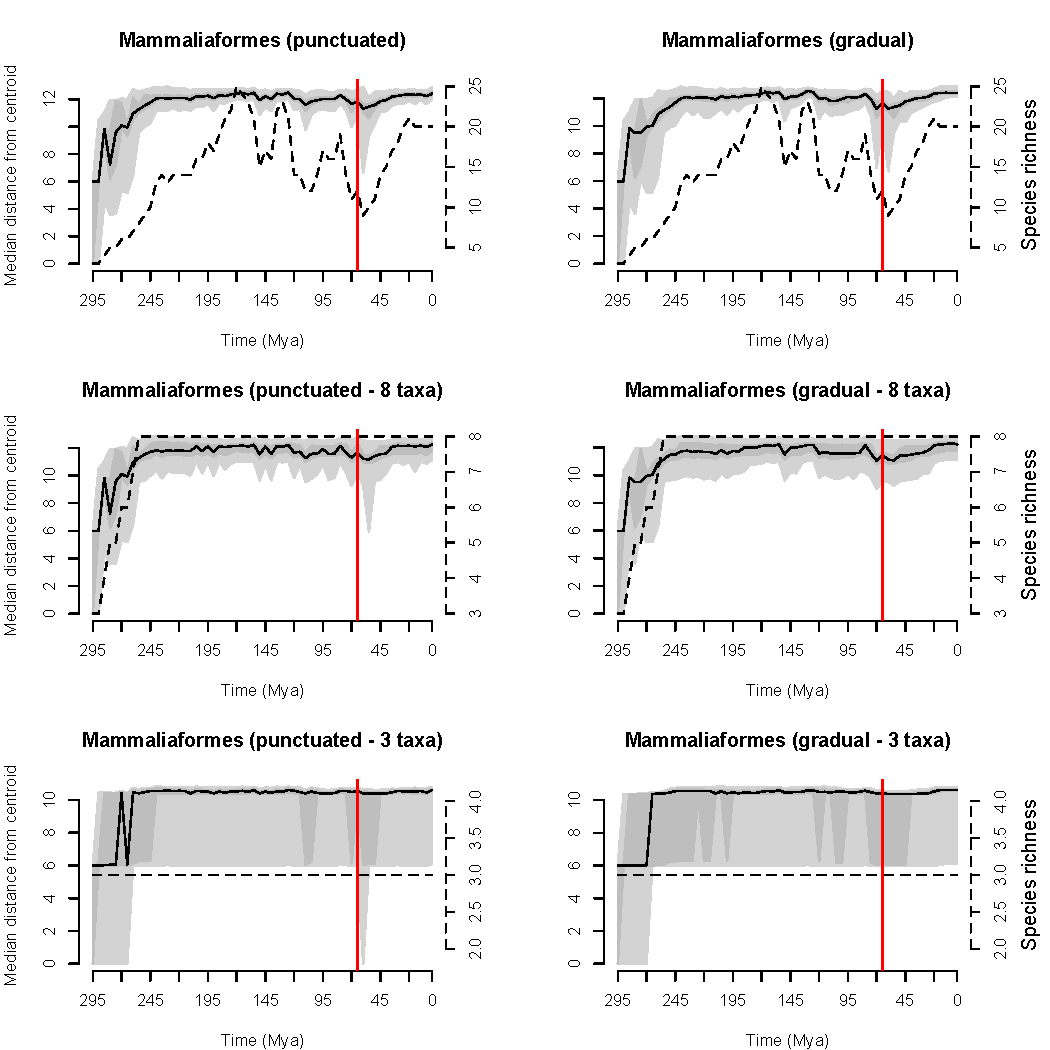
\includegraphics[keepaspectratio=true]{Supplementaries/Figures/STD/Slater_full.pdf}
\caption[Mammaliaformes disparity (rarefied)]{Observed and rarefied variation of disparity through time among Mammaliaformes with a punctuated or gradual evolution model. The x axis represents the time in Million of years ago (relationships among lineages
Ma). The y axis represents the disparity measured as the median distance from centroid per sub-sample. The solid black lines is the mean disparity; the confidence intervals (CI) are represent by the grey polygons (50\% CI in dark grey and 95\% CI in light grey). The dashed line represent the species richness in each sub-sample (values are reported on the right hand side of each graphs). The red vertical line represents the K-Pg boundary (66 relationships among lineages
Ma).}
\label{Supp_Mammaliaformes_rarefied}
\end{figure}

\begin{figure}
\centering
    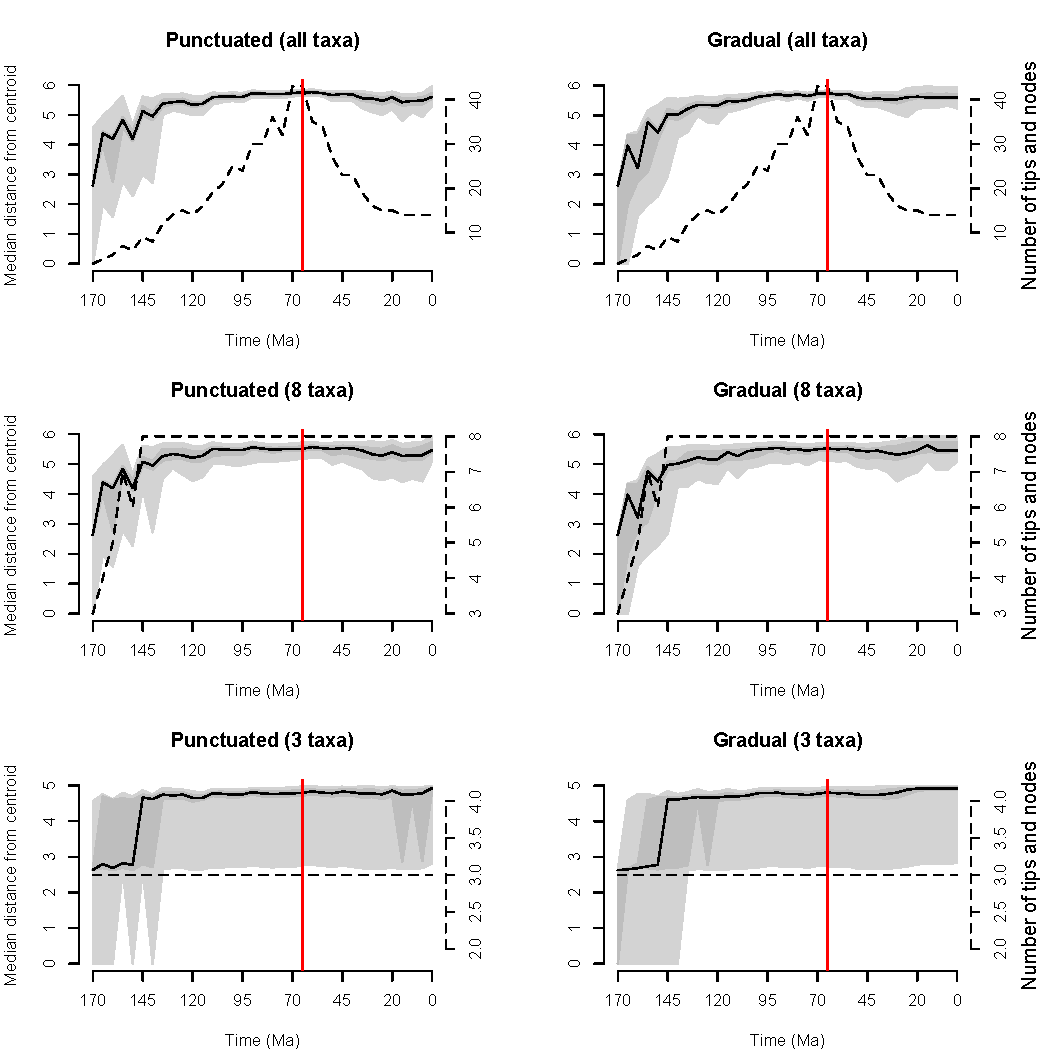
\includegraphics[keepaspectratio=true]{Supplementaries/Figures/STD/Rarefaction-beck.pdf}
\caption[Eutheria disparity (rarefied)]{Variations of disparity through time among Eutheria with a punctuated or gradual evolution model for different number of taxa (rarefaction). The x axis represents the time in Million of years ago (relationships among lineages
Ma). The y axis represents the disparity measured as the median distance from centroid per sub-sample. The solid black lines is the mean disparity; the confidence intervals (CI) are represent by the grey polygons (50\% CI in dark grey and 95\% CI in light grey). The dashed line represent the species richness in each sub-sample (values are reported on the right hand side of each graphs). The red vertical line represents the K-Pg boundary (66 relationships among lineages
Ma).}
\label{Supp_Eutheria_rarefied}
\end{figure}

\newpage
\section{Comparison of different disparity metrics and time sampling methods.}
This section (Fig \ref{Supp_disparity_all_Mammaliaformes}, \ref{Supp_disparity_all_Eutheria}, \ref{Supp_disparity_all_Mammaliaformes_rarefied} and \ref{Supp_disparity_all_Eutheria_rarefied}) contains the results of the variation of disparity through time for the Mammaliaformes and Eutheria dataset with all the disparity metrics and methods for sampling disparity through time.
The different disparity metric are the median distance from centroid (see methods section in Chapter \ref{chap:STD_paper}) as well as the sum and products of ranges and variances of the cladisto-space dimensions \cite{Wills1994}.
The different time sampling methods are:
\begin{enumerate}
\item \textbf{Intervals (tips only)}.
We selected every tip present at every stages from the early Middle Jurassic (Bajocian, starting at 170.3 Ma) to the present.
We collapsed together every stage containing less than 3 tips so that every time interval contained at least 3 tips. Note that some tips where present in multiple stages due to their occurrence data (see methods section in Chapter \ref{chap:STD_paper}).
\item \textbf{Intervals (tips and nodes)}.
We selected every stage tips and nodes present at every stages from the early Middle Jurassic (Bajocian, starting at 170.3 Ma) to the present.
We collapsed together every stage containing less than 3 elements (tips and/or nodes).
\item \textbf{Slices (punctuated)}.
These are the results presented in the main text where the cladisto-space is sampled every 5 Ma and evolution between each subsample is assumed to be punctuated (randomly selecting either data from the descendant or the ancestor when slicing through a branch; see methods section in Chapter \ref{chap:STD_paper}).
\item \textbf{Slices (punctuated: acctran)}.
Similar as the slices (punctuated) method but data is always selected from the descendant (see methods section in Chapter \ref{chap:STD_paper}).
\item \textbf{Slices (punctuated: deltran)}.
Similar as the slices (punctuated) method but data is always selected from the ancestor (see methods section in Chapter \ref{chap:STD_paper}).
\item \textbf{Slices (gradual)}.
These are the results presented in the main text where the cladisto-space is sampled every 5 Ma and evolution is assumed to be gradual (data is selected from the descendant or the ancestor based on branch length; see methods section in the main text for details).
\end{enumerate}
We also rarefied both datasets for all the metrics and all the methods using the minimum of 3 taxa for the interval methods and 8 taxa for the slices methods.

\begin{landscape}
\begin{figure}[!htbp]
\centering
    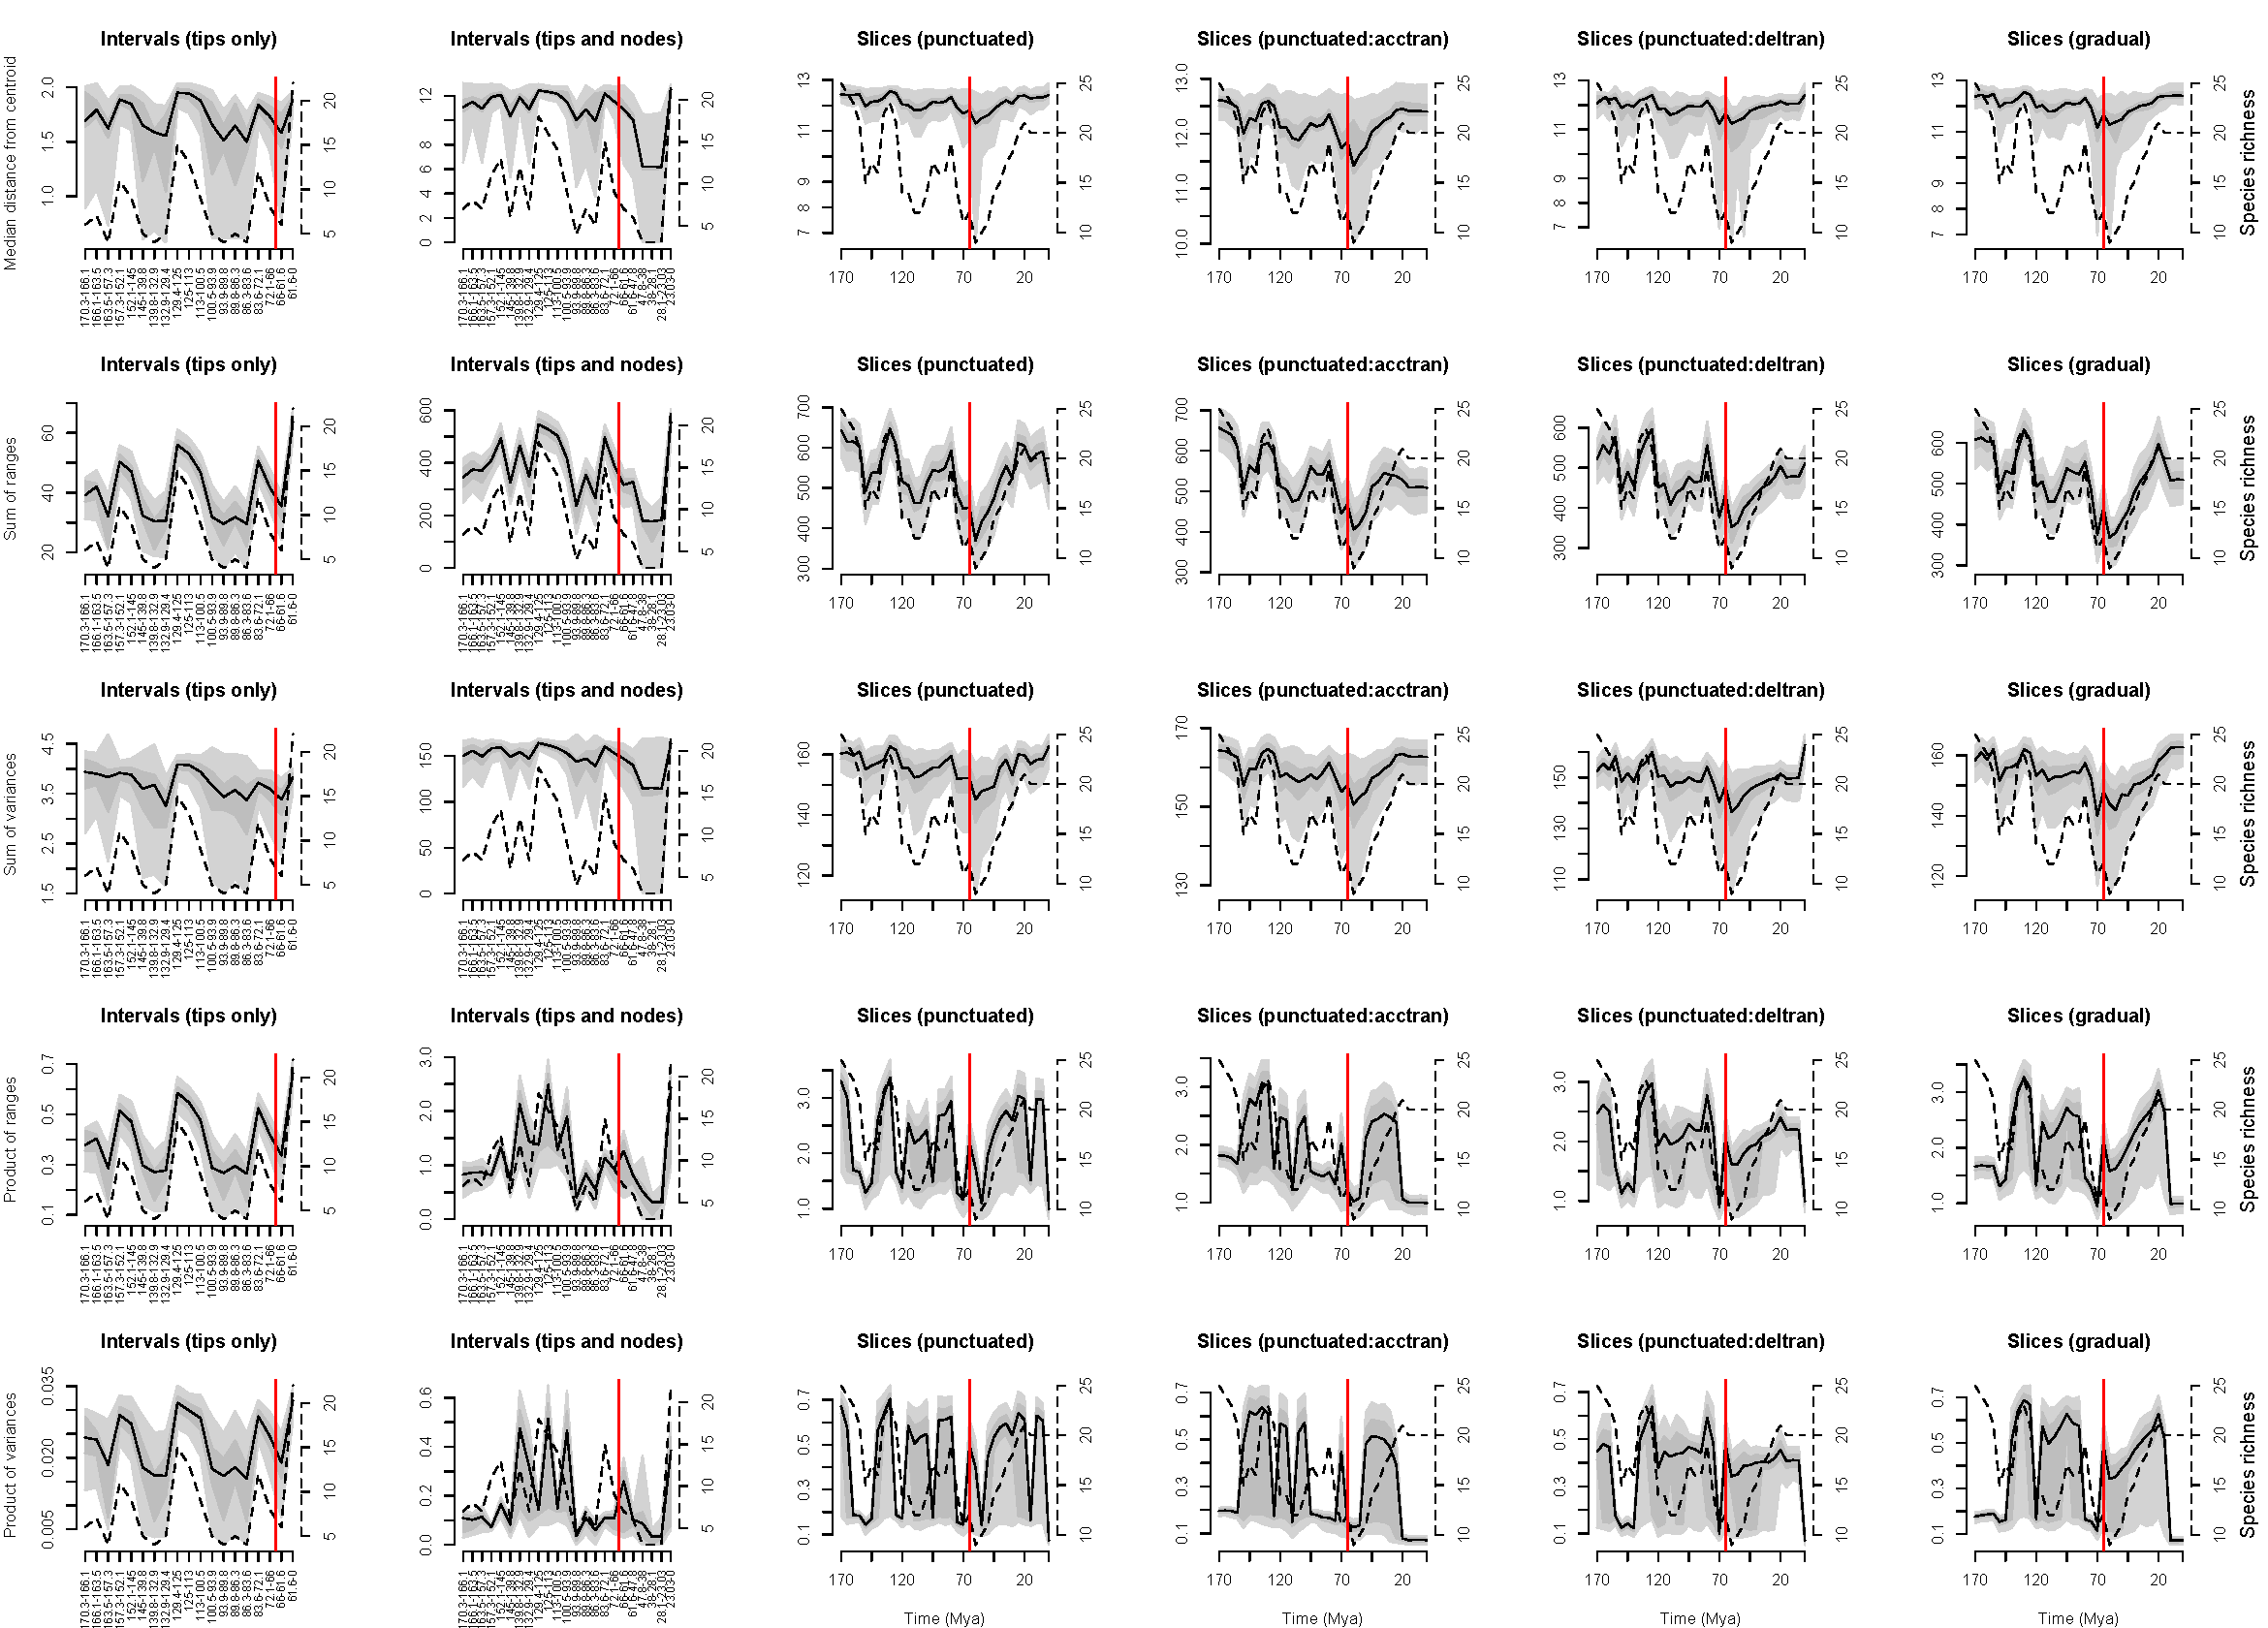
\includegraphics[width=\textwidth,height=\textheight,keepaspectratio]{Supplementaries/Figures/STD/Mammaliaformes_all_methods.pdf}
\caption[Comparison of all the disparity metrics and all the time series methods for Mammaliaformes]{Variations of disparity through time among Mammaliaformes with disparity measurements and methods for sampling disparity through time. The x axis represents the time in Million of years ago (relationships among lineages
Ma). The y axis represents the disparity measured as the median distance from centroid per sub-sample. The solid black lines is the mean disparity; the confidence intervals (CI) are represent by the grey polygons (50\% CI in dark grey and 95\% CI in light grey). The dashed line represent the species richness in each sub-sample (values are reported on the right hand side of each graphs). The red vertical line represents the K-Pg boundary (66 relationships among lineages
Ma).}
\label{Supp_disparity_all_Mammaliaformes}
\end{figure}
\end{landscape}

\begin{landscape}
\begin{figure}[!htbp]
\centering
    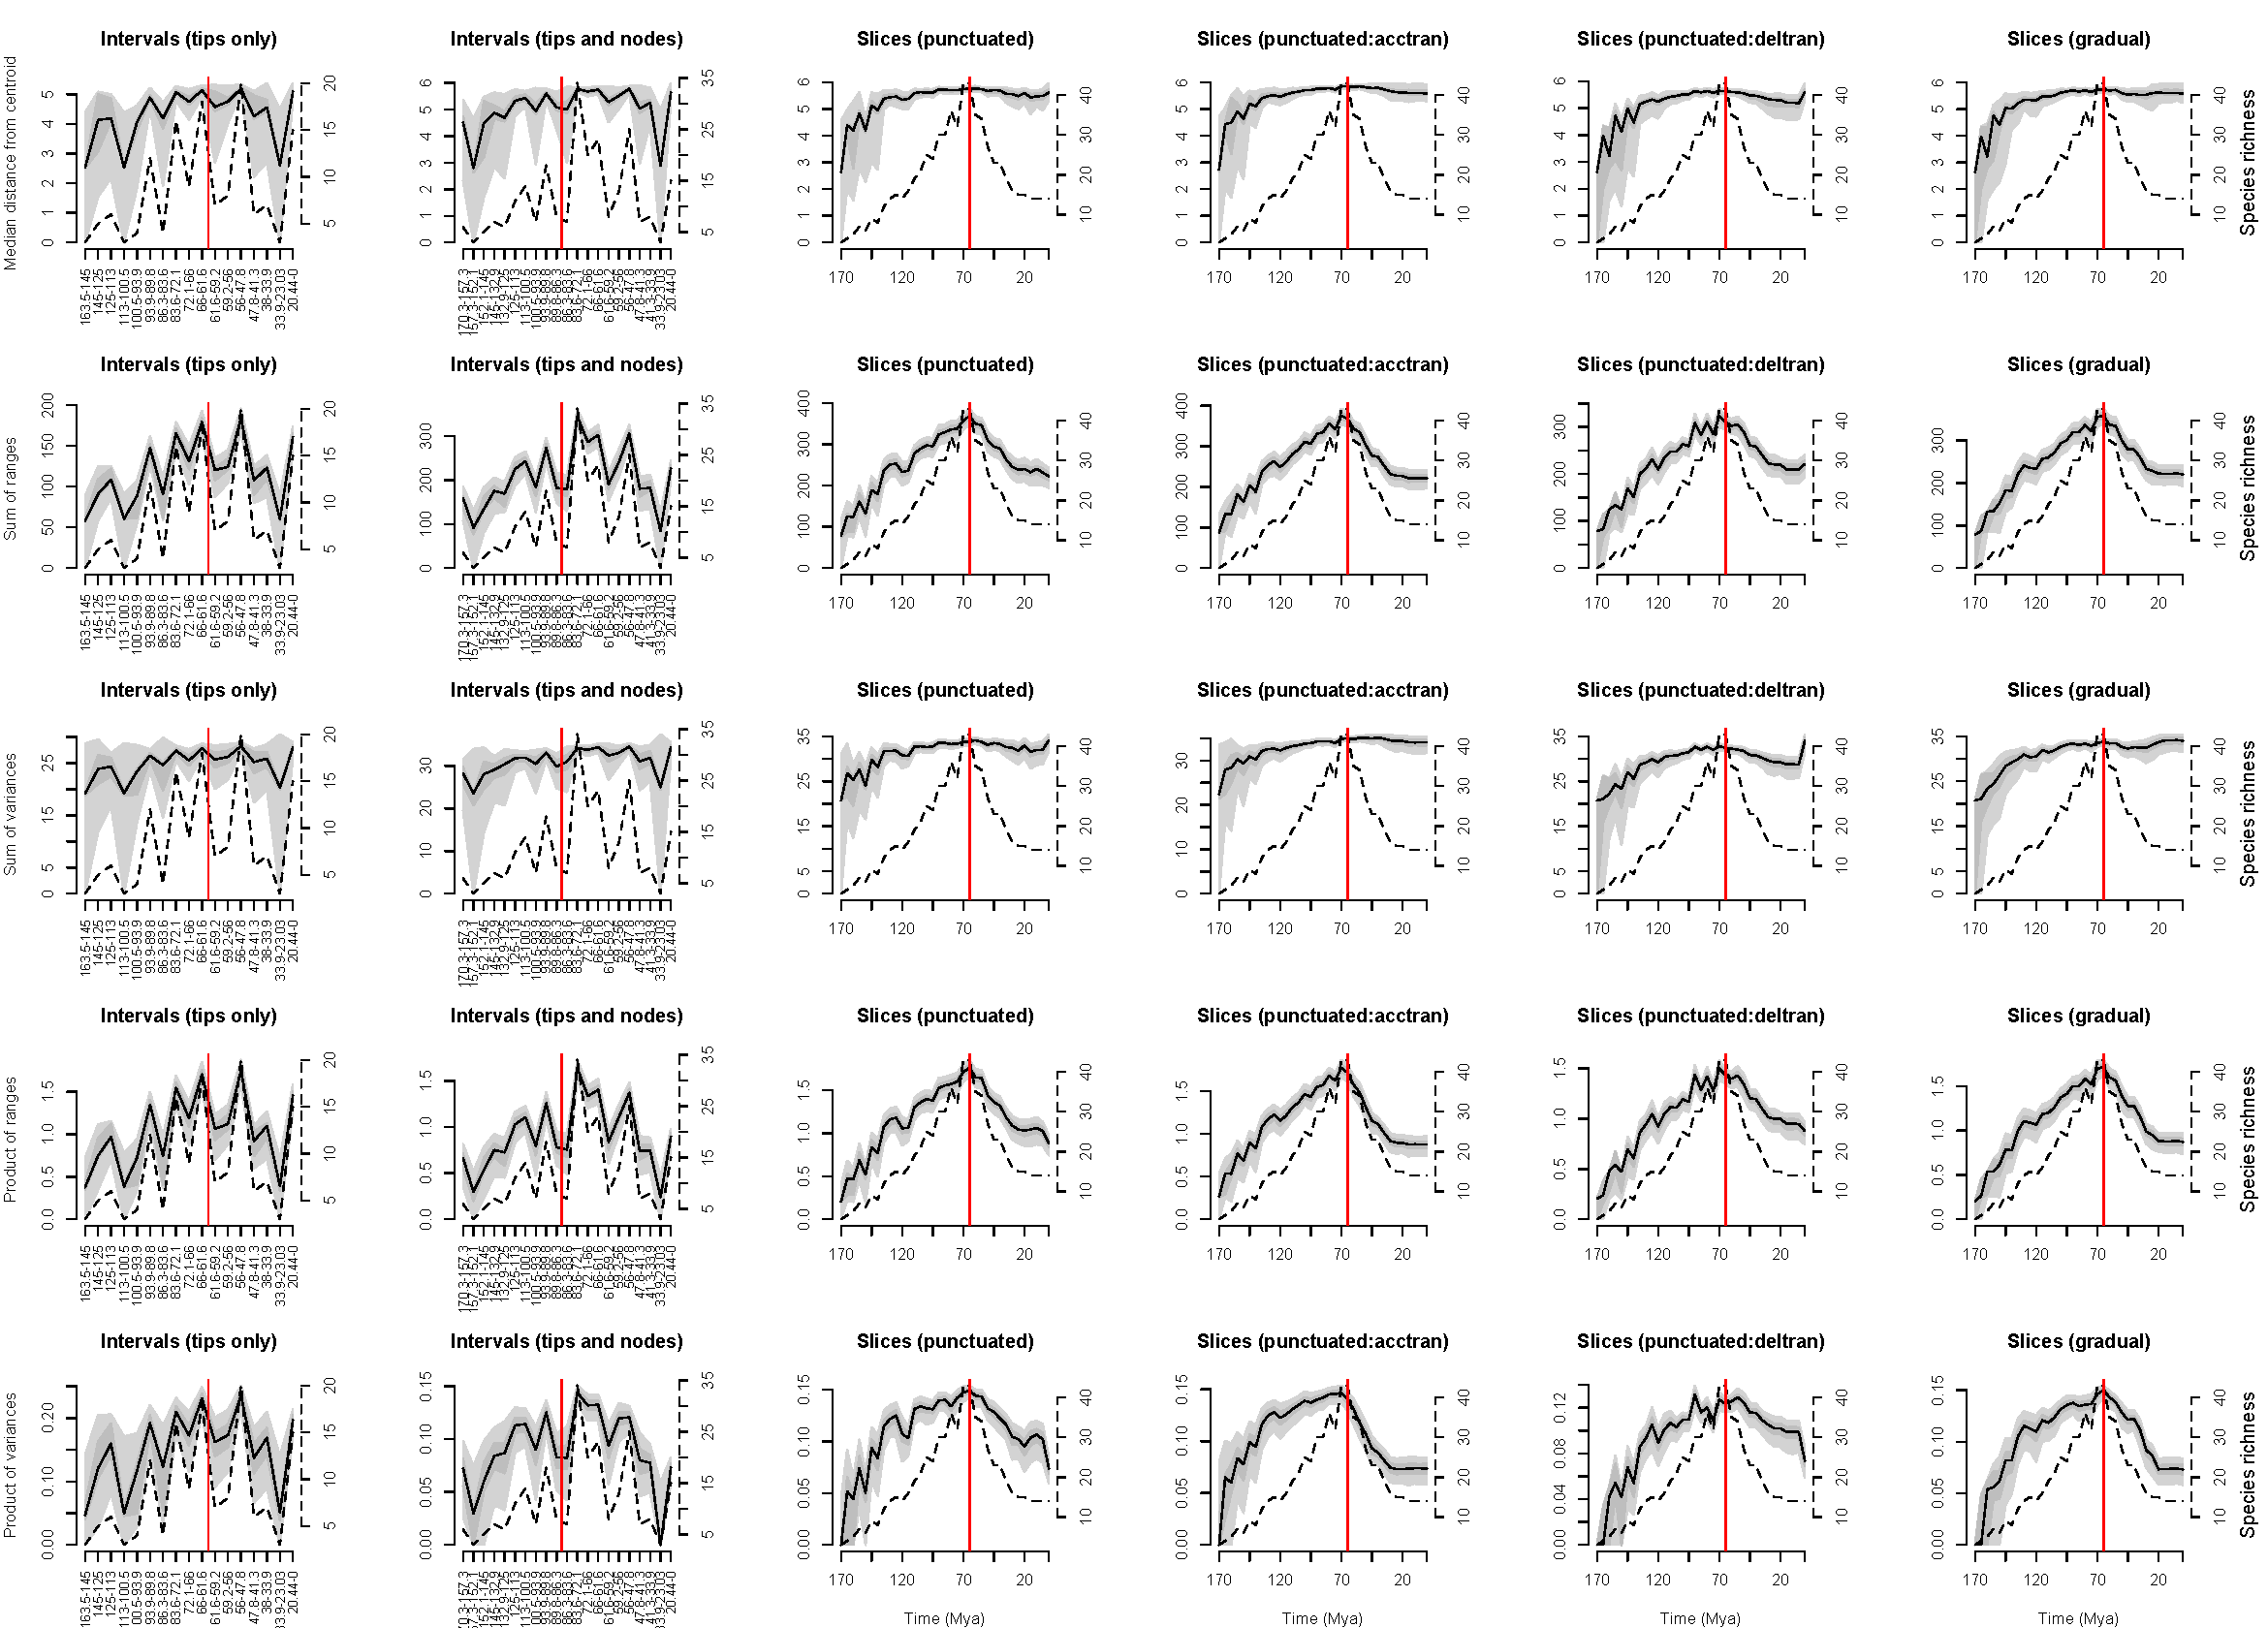
\includegraphics[width=\textwidth,height=\textheight,keepaspectratio]{Supplementaries/Figures/STD/Eutheria_all_methods.pdf}
\caption[Comparison of all the disparity metrics and all the time series methods for Eutheria]{Variations of disparity through time among Eutherian with disparity measurements and methods for sampling disparity through time. The x axis represents the time in Million of years ago (relationships among lineages
Ma). The y axis represents the disparity measured as the median distance from centroid per sub-sample. The solid black lines is the mean disparity; the confidence intervals (CI) are represent by the grey polygons (50\% CI in dark grey and 95\% CI in light grey). The dashed line represent the species richness in each sub-sample (values are reported on the right hand side of each graphs). The red vertical line represents the K-Pg boundary (66 relationships among lineages
Ma).}
\label{Supp_disparity_all_Eutheria}
\end{figure}
\end{landscape}



\begin{landscape}
\begin{figure}[!htbp]
\centering
    \includegraphics[width=\textwidth,height=\textheight,keepaspectratio]{Supplementaries/Figures/STD/Mammaliaformes_all_methods_rarefied.pdf}
\caption[Comparison of all the disparity metrics and all the time series methods for Mammaliaformes (rarefied)]{Variations of disparity through time among Mammaliaformes with disparity measurements and methods for sampling disparity through time (rarefied with 3 taxa for the interval method and 8 taxa for the slice method). The x axis represents the time in Million of years ago (relationships among lineages
Ma). The y axis represents the disparity measured as the median distance from centroid per sub-sample. The solid black lines is the mean disparity; the confidence intervals (CI) are represent by the grey polygons (50\% CI in dark grey and 95\% CI in light grey). The dashed line represent the species richness in each sub-sample (values are reported on the right hand side of each graphs). The red vertical line represents the K-Pg boundary (66 relationships among lineages
Ma).}
\label{Supp_disparity_all_Mammaliaformes_rarefied}
\end{figure}
\end{landscape}

\begin{landscape}
\begin{figure}[!htbp]
\centering
    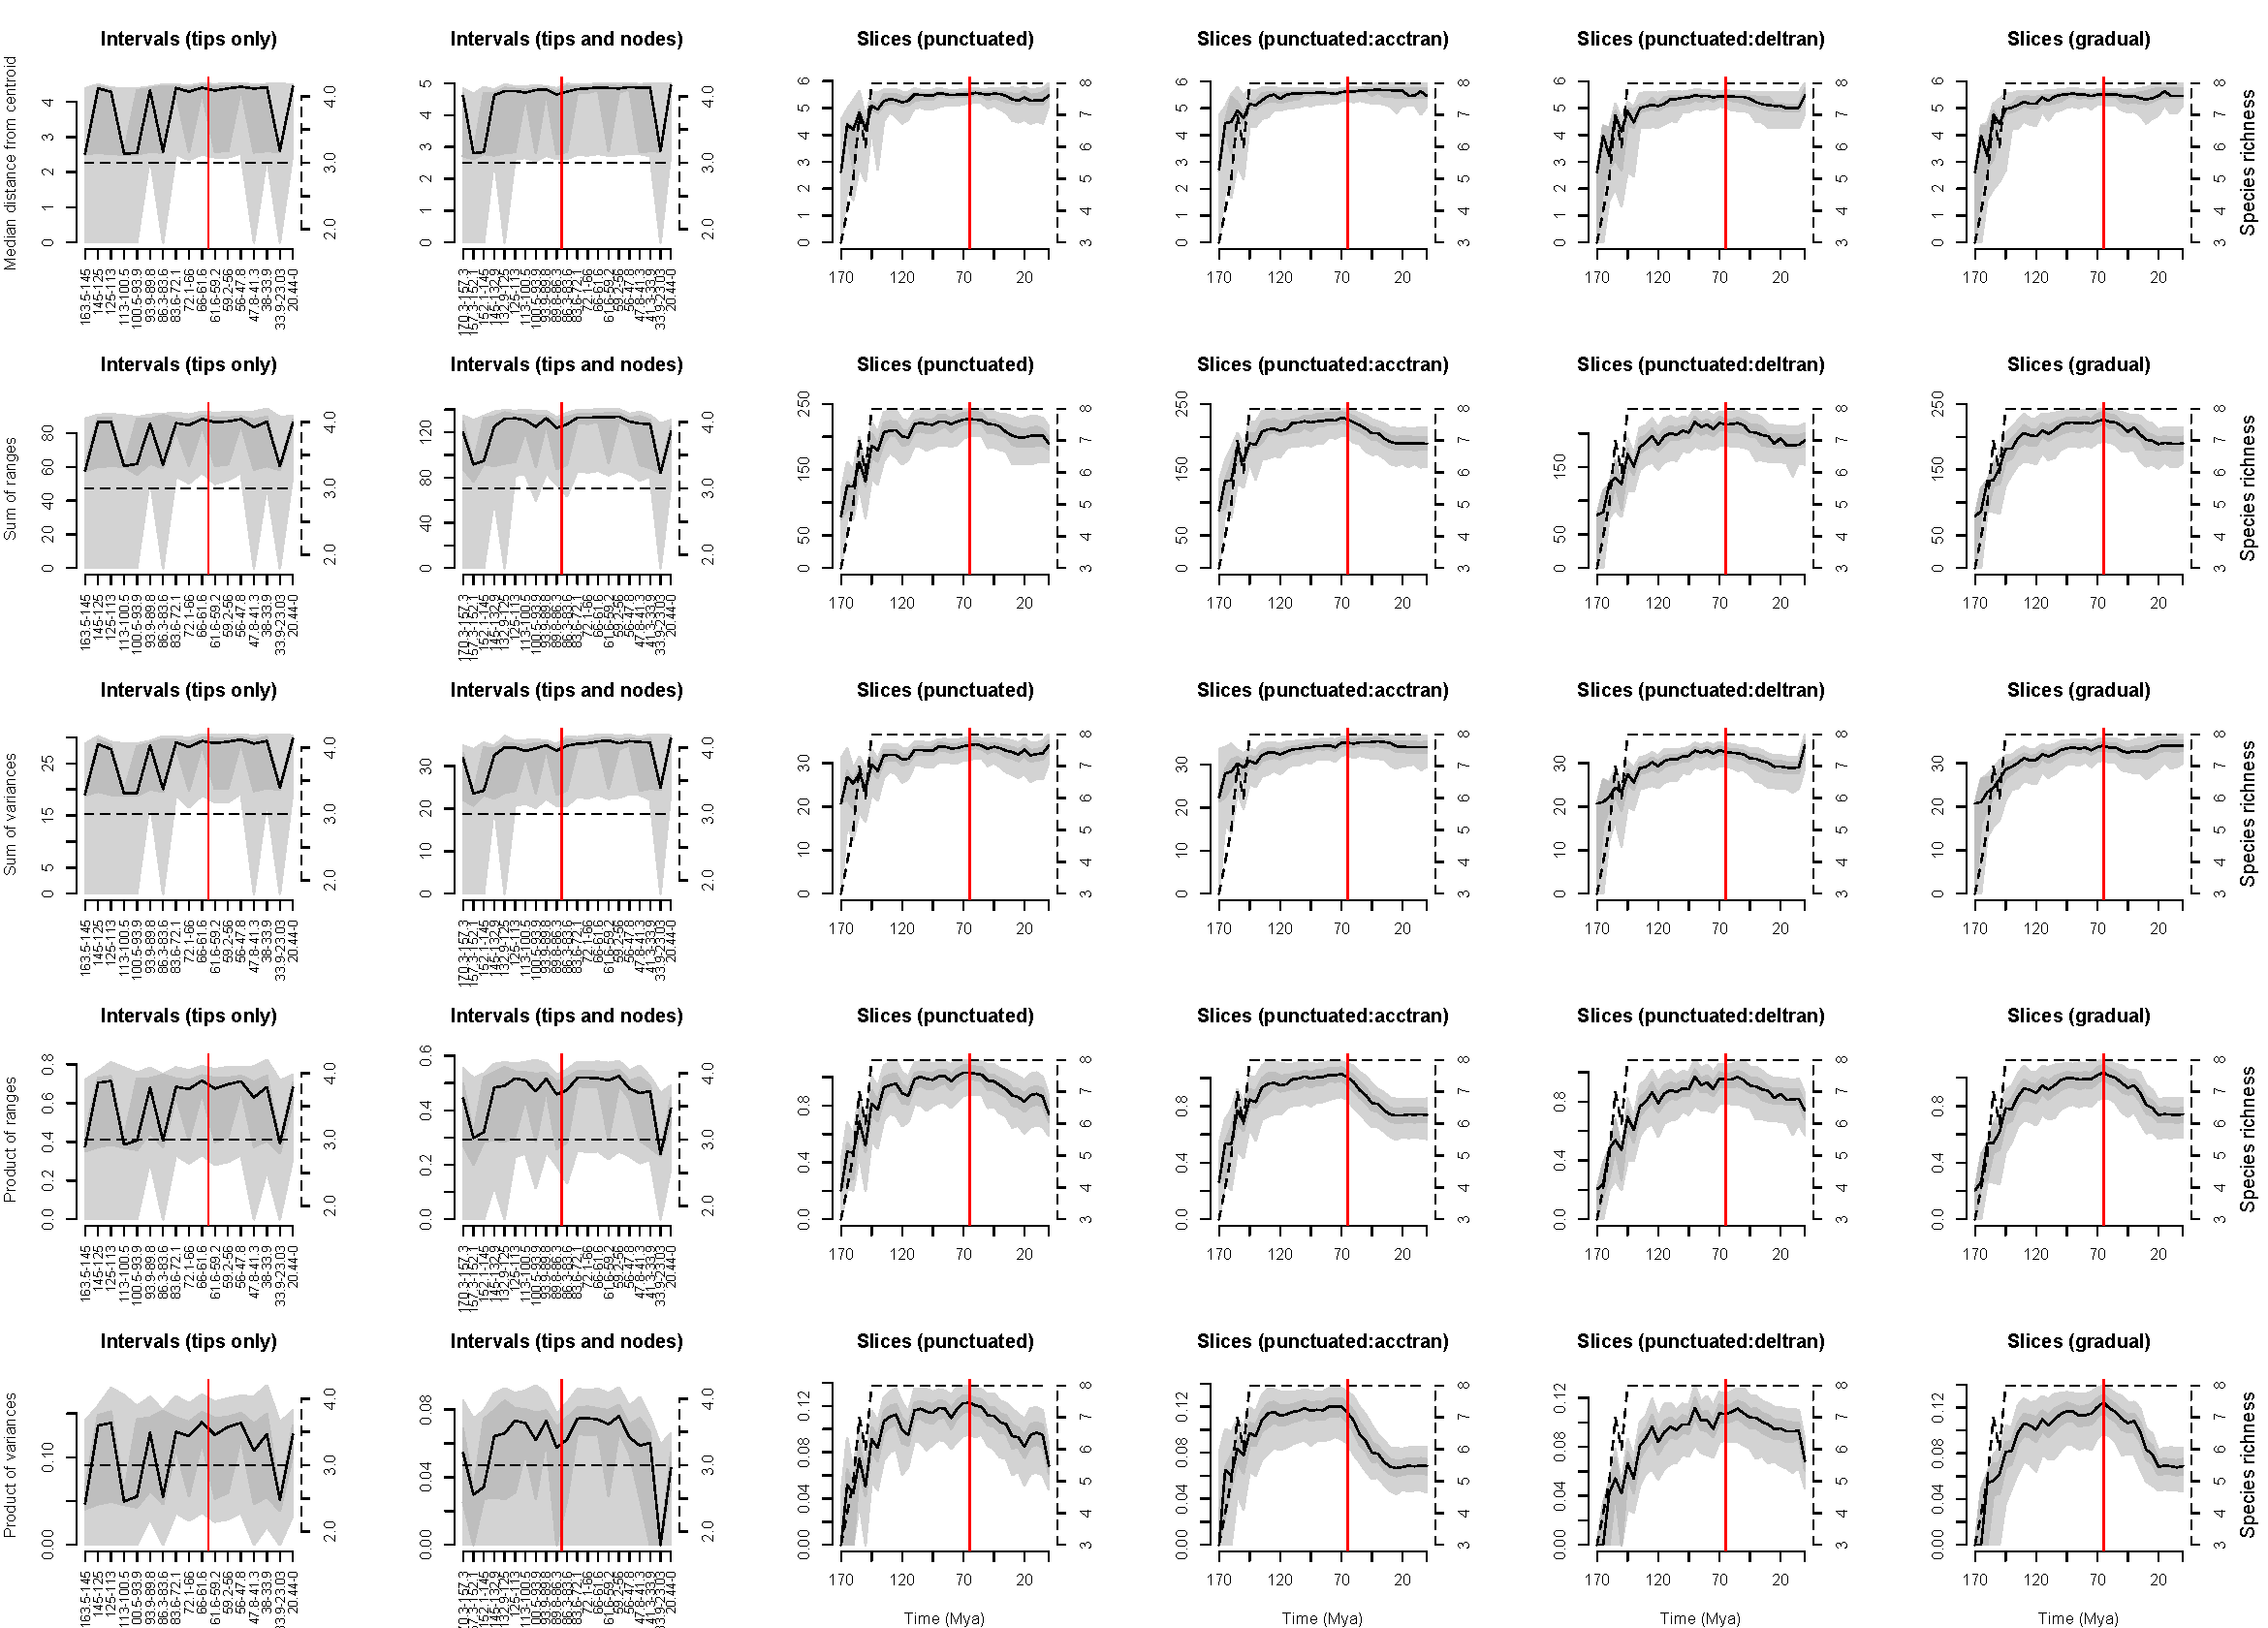
\includegraphics[width=\textwidth,height=\textheight,keepaspectratio]{Supplementaries/Figures/STD/Eutheria_all_methods_rarefied.pdf}
\caption[Comparison of all the disparity metrics and all the time series methods for Eutheria (rarefied)]{Variations of disparity through time among Eutherian with disparity measurements and methods for sampling disparity through time (rarefied with 3 taxa for the interval method and 8 taxa for the slice method). The x axis represents the time in Million of years ago (relationships among lineages
Ma). The y axis represents the disparity measured as the median distance from centroid per sub-sample. The solid black lines is the mean disparity; the confidence intervals (CI) are represent by the grey polygons (50\% CI in dark grey and 95\% CI in light grey). The dashed line represent the species richness in each sub-sample (values are reported on the right hand side of each graphs). The red vertical line represents the K-Pg boundary (66 relationships among lineages
Ma).}
\label{Supp_disparity_all_Eutheria_rarefied}

\end{figure}
\end{landscape}